\documentclass[9pt]{beamer}
%----------------------------------------------------------
% Стиль презентации (выбрать понравившийся)
\usetheme{bmstu}
%------------------------------------------
% определения значений стандартных параметров
%----------------------------------------%
% общие определения
\newcommand{\UpperFullOrganisationName}{Министерство науки и высшего образования Российской Федерации}
\newcommand{\ShortOrganisationName}{МГТУ~им.~Н.Э.~Баумана}
\newcommand{\FullOrganisationName}{федеральное государственное бюджетное образовательное\newline учреждение высшего профессионального образования\newline <<Московский государственный технический университет имени Н.Э.~Баумана\newline (национальный исследовательский университет)>> (\ShortOrganisationName)}
\newcommand{\OrganisationAddress}{105005, Россия, Москва, ул.~2-ая Бауманская, д.~5, стр.~1}
%----------------------------------------%
\newcommand{\gitlabdomain}{sa2systems.ru:88}
%----------------------------------------------------------
\newcommand{\doctypesid}{kp} % vkr (выпускная квалификационная работа) / kp (курсовой проект) / kr (курсовая работа) / nirs (научно-исследовательская работа студента) / nkr (научно-квалификационная работа)

% Тема должна быть сформулирована так, чтобы рассказать, о чем работа, но сделать это так, чтобы у читателя возникло желание читать аннота-цию. При формулировке темы не следует стараться рассказать о работе всё. Пример корректной темы: "Математическое моделирование процесса размножения медуз в Южно-Китайском море". Пример некорректной темы: "Применение модели SIS для моделирования процесса размножения медуз в Южно-Китайском море с использованием метода Рунге-Кутты и многопроцессорных вычислительных систем".
\newcommand{\Title}{Разработка механизма вывода типов с использованием системы типов Хиндли-Милнера}%{}
\newcommand{\TitleSource}{кафедра} % кафедра, предприятие, НИР, НИР кафедры, заказ организации

\newcommand{\SubTitle}{по дисциплине <<Модели и методы анализа проектных решений>>} % Методы оптимизации
\newcommand{\faculty}{<<Робототехника и комплексная автоматизация>>}
\newcommand{\facultyShort}{РК}
\newcommand{\department}{<<Системы автоматизированного проектирования (РК-6)>>}
\newcommand{\departmentShort}{РК-6}

\newcommand{\Author}{Никитин В.Л.}
\newcommand{\AuthorFull}{Никитин Владимир Леонидович}
\newcommand{\ScientificAdviserPosition}{доктор физико-математических наук}    % Должность научного руководителя
\newcommand{\ScientificAdviser}{Соколов А.П.}    % Научный руководитель
\newcommand{\ConsultantA}{Соколов А.П.}                % Консультант 1
% \newcommand{\ConsultantB}{@Фамилия~И.О.@}				% Консультант 2
\newcommand{\Normocontroller}{Грошев~С.В.}        % Нормоконтролёр
\newcommand{\group}{РК6-75Б}
\newcommand{\Semestr}{осенний семестр} % Например: осенний семестр или весенний семестр
\newcommand{\BeginYear}{2023}
\newcommand{\Year}{2024}
\newcommand{\Country}{Россия}
\newcommand{\City}{Москва}
\newcommand{\TaskStatementDate}{<<\underline{\textit{01}}>> \underline{октября} \Year~г.} %Дата выдачи задания

\newcommand{\depHeadPosition}{Заведующий кафедрой}        % Должность руководителя подразделения
\newcommand{\depHeadName}{А.П.~Карпенко}        % Должность руководителя подразделения

% Цель выполнения 
\newcommand{\GoalOfResearch}{реализация системы вывода и проверки типов} % с маленькой буквы и без точки на конце

% Объектом исследования называют то, что исследуется в работе. Например, для указанной выше темы объектом может быть популяция медуз, но никак ни модель SIS, ни Южно-Китайское море, ни метод моделирования популяции медуз. 
\newcommand{\ObjectOfResearch}{система типов}

% Предмет исследований (уже чем объект, определяется, исходя из задач: формулируется как существительное, как правило, во множественном числе, определяющее "конкретный объект исследований" среди прочих в рамках более общего)
\newcommand{\SubjectOfResearch}{система типов Хиндли-Милнера}

% Основная задача, на решение которой направлена работа
\newcommand{\MainProblemOfResearch}{реализация алгоритма вывода типов на основе выбранной системы типов}

% Выполненные задачи
\newcommand{\SubtasksPerformed}{%
    В результате выполнения работы:
    \begin{inparaenum}[1)]
        \item спроектировано представление абстрактного синтаксического дерева в компиляторе;
        \item реализован семантический анализатор;
        \item показано, что компилятор успешно может вывести тип функции
    \end{inparaenum}}

% Ключевые слова (представляются для обеспечения потенциальной возможности индексации документа)
\newcommand{\keywordsru}{%
    теория типов, языки программирования, компиляторы, фукнциональное программирование, система типов Хиндли-Милнера} % 5-15 слов или выражений на русском языке, для разделения СЛЕДУЕТ ИСПОЛЬЗОВАТЬ ЗАПЯТЫЕ
\newcommand{\keywordsen}{%
    type theory, programming languages, compilers, functional programming, Hindley-Milner type system} % 5-15 слов или выражений на английском языке, для разделения СЛЕДУЕТ ИСПОЛЬЗОВАТЬ ЗАПЯТЫЕ

% Краткая аннотация
\newcommand{\Preface}{
	Работа посвящена реализации механизма вывода типов для языка программирования Kodept.
	Программирование выстроено вокруг глубокой математической теории.
	Благодаря этому появляются возможности для оптимизации, развития и улучшения языков посредством применения математики.
	Одним из важных применений является теория типов, которая помогает программисту в написании кода.
	В последнее время все больше и больше языков почерпывают что-то из этой области.
	Применение мощной системы типов позволяет зачастую снизить количество ошибок, возникающих при разработке.
} % с большой буквы с точкой в конце

%----------------------------------------%
% выходные данные по документу
\newcommand{\DocOutReference}{\Author. \Title\xspace\SubTitle. [Электронный ресурс] --- \City: \Year. --- \total{page} с. URL:~\url{https://\gitlabdomain} (система контроля версий кафедры РК6)}

%----------------------------------------------------------


%------------------------------------------
% определения значений стандартных общих параметров для различных документов, в т.ч. различных типов
%----------------------------------------------------------
% Информация о лицензии
\newcommand{\doclicense}{\copyright\xspace}
%\newcommand{\doclicense}{\includegraphics[width=0.1\textwidth]{../common_doc_spec/by.eps}\xspace}%\ccShareAlike
%----------------------------------------------------------
\newcommand{\doctextlicense}{\copyright\xspace} % Copyright ©
%\newcommand{\doctextlicense}{CC BY 4.0}% \ccAttribution
%----------------------------------------%
% общие определения
\newcommand{\UpperFullOrganisationName}{Министерство науки и высшего образования Российской Федерации}
\newcommand{\ShortOrganisationName}{МГТУ~им.~Н.Э.~Баумана}
\newcommand{\FullOrganisationName}{Московский государственный технический университет имени Н.Э.~Баумана}
\newcommand{\OrganisationAddress}{105005, Россия, Москва, ул.~2-ая Бауманская, д.~5, стр.~1}
%----------------------------------------%
\newcommand{\gitlabdomain}{gitlab.sa2systems.ru}
%----------------------------------------%
\newcommand{\faculty}{<<Робототехники и комплексной автоматизации>>}
\newcommand{\facultyShort}{РК}
\newcommand{\department}{<<Системы автоматизированного проектирования (РК-6)>>}
\newcommand{\departmentShort}{РК-6}
\newcommand{\departmentcloud}{\href{https://archrk6.bmstu.ru}{https://archrk6.bmstu.ru}}
%----------------------------------------------------------


%------------------------------------------
% общая кастомизируемая преамбула для презентаций
%----------------------------------------------------------
% Сохранение метаданных в PDF об авторе документа
\expandafter\hypersetup{%
		pdftitle={\Title},    	% title
		pdfauthor={\Author},    % author
		pdfcopyright={\doctextlicense, \begdate -- \Year, \Author. Все права защищены.},% -- \today,
		pdfsubject={\Title},   % subject of the document
%		pdfcreator={\pdftexbanner},   % creator of the document
		pdfpublisher={\department, \ShortOrganisationName},
		pdfcaptionwriter={\Author},
		pdfproducer={\Author, \begdate -- \Year, \ShortOrganisationName}, % producer of the document
		pdfkeywords={\keywordsru, \keywordsen}, % producer of the document
}
%----------------------------------------------------------
% final - удаляет все всплывающие комментарии
%\usepackage[author={\Author},opacity=0.1, final]{pdfcomment}
\usepackage[opacity=0.1]{pdfcomment}
%----------------------------------------------------------
\usepackage{tikz}
\usetikzlibrary{tikzmark}
\usetikzlibrary{matrix,automata,positioning,arrows,arrows.meta,graphs}
\usetikzlibrary{trees,topaths}
\usetikzlibrary{calc, circuits.ee.IEC}
\usetikzlibrary{patterns,decorations.pathmorphing,decorations.markings}
%----------------------------------------------------------

%------------------------------------------
% дополнительные параметры, имеющие отношение к данному документу
%----------------------------------------------------------
\newcommand\ddfrac[2]{\frac{\displaystyle #1}{\displaystyle #2}}
\newcommand\T{\textup{T}}
\def\argmin{\operatornamewithlimits{argmin}}
\def\argmax{\operatornamewithlimits{argmax}}
\def\diag{\operatornamewithlimits{diag}}
\def\dep{\operatornamewithlimits{dep}}
%----------------------------------------------------------
\newcommand{\bvec}[1]{\mbox{\mathversion{bold}${#1}$}}
\newcommand{\periodichnost}[1]{[\hspace{-2pt}[#1]\hspace{-2pt}]}
\newcommand{\volna}[1]{\mathop{#1}\limits\_{\sim}}
\newcommand{\crujok}[1]{#1}
\newcommand{\driv}[2]{\frac{d#1}{d#2}}
\newcommand{\pdriv}[2]{\frac{\partial #1}{\partial #2}}
\newcommand{\uparr}[1]{\overrightarrow{#1}}
\newcommand{\intThreeD}[1]{\hspace{6pt}\mathop{\int\hspace{-17pt}\int\hspace{-17pt}\int}\limits\_{#1}\hspace{6pt}}
\newcommand{\intTwoD}[1]{\hspace{6pt}\mathop{\int\hspace{-17pt}\int}\limits\_{\hspace{-6pt}#1}}
\newcommand{\mbf}[1]{\boldsymbol{#1}}
\renewcommand{\H}{\operatornamewithlimits{\mathit{H}}}
%----------------------------------------------------------
\newcommand{\multirowbox}[2]
{
   \parbox{#1}{\smallskip #2 \smallskip}
}
%----------------------------------------------------------

\declaretheorem[
  style=thrmstyle,
  title=Замечание,
  refname={замечание,замечания},
  Refname={Замечание,Замечания}
]{remark}

\theoremstyle{thrmstyle}

%\newtheorem{question}{Вопрос}
%\newtheorem{approval}{Утверждение}
%\newtheorem{demand}{Требование}
%\newtheorem{statement}{Утверждение}
%\newtheorem{syntax}{Синтаксис}
\let\definition\relax
\newtheorem{definition}{Определение}
%\newtheorem{designation}{Обозначение}
%\newtheorem{property}{Свойство}
\newtheorem{task}{Задача}
%\newtheorem{mathmod}{Математическая модель}
%\newtheorem{mytheorem}{Теорема}

%----------------------------------------------------------
\hyphenation{супер-ком-пью-тер-ный супер-ком-пью-тер-ное вы-со-ко-произ-во-ди-тель-ный}
%----------------------------------------------------------
\newcommand\MyProcess[3]
{
%\begin{tabular}{p{0.1\textwidth}p{0.9\textwidth}}
%&
\begin{lstlisting}[caption={#1}, label={#2}, language=ALGO, basicstyle=\small]
#3
\end{lstlisting}			
%\end{tabular}
}
%----------------------------------------------------------
\newcommand\myquote[2]{%
\textit{``#1''}
\begin{flushright}
\textcolor{gray}{#2}
\end{flushright}
}
%----------------------------------------------------------
\newcommand{\mydescr}[1]{%

\colorbox{black!5}{\parbox{0.7\textwidth}{\smaller[1]\textit{#1}}}
}
%----------------------------------------------------------
% вёрстка в две колонки
\newcommand\cols[4]
{\smaller[1]%
		\begin{columns}
		\begin{column}{#1}
    #2
		\end{column}
		\begin{column}{#3}
		#4
		\end{column}
		\end{columns}}
%----------------------------------------------------------
% вёрстка в две колонки двух блоков с itemize
\newcommand\colsblocks[4]
{\smaller[1]%
		\begin{columns}
		\begin{column}{0.5\textwidth}
		\begin{block}{#1}
		\begin{itemize}
			#2
		\end{itemize}
		\end{block}
		\end{column}
		\begin{column}{0.5\textwidth}
		\begin{block}{#3}
		\begin{itemize}
			#4
		\end{itemize}
		\end{block}
		\end{column}
		\end{columns}}
%----------------------------------------------------------
%\usepackage{ifthen}
%%----------------------------------------------------------
%\usepackage{totcount}
%%----------------------------------------------------------
%%\newboolean{shortversion}
%% #1 - current \doctype
%% #2 - destination document
%% #3 - text
%\newcommand{\myconditionaltext}[3]%
%{%
	%\ifthenelse{\equal{#1}{avtoreferat}\AND\equal{#2}{avtoreferat}}{#3}{}% short version
	%\ifthenelse{\equal{#1}{avtoreferat}\AND\equal{#2}{thesis}}{}{}% short version
	%\ifthenelse{\equal{#1}{avtoreferat}\AND\equal{#2}{presentation}}{}{}% short version
	%\ifthenelse{\equal{#1}{thesis}\AND\equal{#2}{presentation}}{}{}% short version
	%\ifthenelse{\equal{#1}{thesis}\AND\equal{#2}{thesis}}{#3}{}% short version
	%\ifthenelse{\equal{#1}{presentation}\AND\equal{#2}{presentation}}{#3}{}% short version
	%\ifthenelse{\equal{#1}{presentation}\AND\equal{#2}{thesis}}{\pdfcomment{#3}}{}% short version
%}

%----------------------------------------------------------
% #1 - Короткое название практики
% #2 - Короткое описание
% #3 - Назначение в форме itemize
% #4 - LaTeX код
\newcommand{\bestpractice}[4]{%
\subsection{#1}
\begin{frame}%[fragile]

{\smaller[1]
#2}

\begin{columns}[t]

\begin{column}{0.5\textwidth}
\begin{block}{Назначение}
{\smaller[1]%
#3}
\end{block}
\end{column}

\begin{column}{0.5\textwidth}
\begin{lstlisting}[language={TeX}, basicstyle=\scriptsize]
#4
\end{lstlisting}
\end{column}
\end{columns}

\end{frame}}
%----------------------------------------------------------
\newenvironment{arreqn}[2]
    {\smaller[1]
		\begin{block}{\smaller[1] #1}
    \begin{equation}\label{#2}
    \begin{array}{l}
    }
		{
    \end{array}
    \end{equation}
		\end{block}
    }
%----------------------------------------------------------





%------------------------------------------
% база терминов! 
%----------------------------------------------------------
%Термины и определения по тексту в большинстве случаев выделяются курсивом.

%%%%% для обычных newglossaryentry по умолчанию category==general.
%%%%% для обычных newabbreviation по умолчанию category==abbreviation.
%%%%% команда для создания своей категории \glscategory{<label>}

%\newabbreviation[category=initialism]{aINI}{aINI}{Расширенный формат \href{https://en.wikipedia.org/wiki/INI_file}{INI} (\href{http://sa2systems.ru/svn/public/sa2pdf/comfrm_ugd_AdvancedINI.pdf}{описание в документе <<Соколов А.П., Першин А.Ю. Руководство системного программиста. Формат данных Advanced INI (aINI) // Каркас системы comfrm – 2007-2017 – 18 стр.>>})}

%\newglossaryentry{AI}{name={ActionItem}, description={Функциональная возможность в системе \gls{dcs-gcd}. Понятие, введенное с целью определить абстракции над функциями различных типов, на основе которых возможно расширение функциональных возможностей разрабатываемой программной системы.}}

%\newglossaryentry{slver}{name={Solver}, description={Решатель системы \gls{dcs-gcd}. Регистрируется в таблице \textbf{com.slvrs} БД \gls{gcddb} \gls{dcs-gcd}.}}

\newabbreviation[category=initialism]{PO}{ПО}{Программное обеспечение}
\newabbreviation[category=initialism]{cm}{КМ}{Композиционный материал}
%\newabbreviation[category=initialism]{ASUTP}{АСУ ТП}{Автоматизированная система управления технологическими процессами.}
%\newabbreviation[category=initialism]{chb}{БзЧ}{базовая часть}

%\newglossaryentry{Gij}{name={$G_{ij}$},
	%	symbol={\ensuremath{\mathcal{\nu}}},
%	category=symbol,
%	description={модули сдвига ортотропного материала}}

%\GlsXtrEnableEntryCounting
%{abbreviation}% list of categories to use entry counting
%{2}% trigger value

%\GlsXtrEnableEntryCounting
%{symbol}% list of categories to use entry counting
%{2}% trigger value


%----------------------------------------------------------




%---------------------------------------------
\includeonly{%
chapters/00_intro,
chapters/01_review,
chapters/02_taskstatement,
chapters/03_software,
chapters/XX_conclusion
}
%---------------------------------------------
% выключает разворачивание терминов и аббревиатур при первом использовании в том числе, - всегда термины и аббревиатуры будут выводиться кратко 
\glsunsetall
%----------------------------------------------------------
% Это следует использовать и визуализировать с помощью Dual-side PDF Viewer - dspdfviewer-1.15.1.2)
%\setbeameroption{show notes on second screen=right} % Both
%----------------------------------------------------------
%\setbeameroption{hide notes} % Only slides
%\setbeameroption{show only notes} % Only notes
%\setbeameroption{show notes} % Both
%\setbeamertemplate{note page}{\pagecolor{yellow!5}\insertnote}
%---------------------------------------------
\begin{document}
%---------------------------------------------
% создание стандартной титульной страницы
%----------------------------------------------------------
% Определение значений параметров для формирования титульной страницы
\institute{\FullOrganisationName}
\title{\presentationtitle}
\subtitle{\small
\textit{\SubTitle}\vspace{5pt} \hfill\break
\raggedright\noindent Место проведения: \textit{\eventplace} \hfill\break
\raggedright\noindent Продолжительность: \textit{\eventduration}}
\author{\AuthorFull}%[\Author]
\date[\city\enskip\year]{\scriptsize\conferenceperiod}
%----------------------------------------------------------
% Создание МГТУ-шной титульной страницы
\ifthenelse{\equal{\titlepagestyle}{brief}}{%
\setbeamercolor{background canvas}{bg=bblue}
\begin{frame}[t]
\nobibliography{bibliography}

    \begin{beamercolorbox}[wd=15cm,leftskip=-0.2cm,sep=5pt]{pretitle}
      \myalssector\textbf{\insertinstitute}%\par
    \end{beamercolorbox}

%    \vspace{1.5cm}
    \vskip\titleheaderskip%
    \begin{beamercolorbox}[wd=11cm,leftskip=-0.4cm,sep=5pt]{pretitle}
     \myalssector\Huge\textbf{\inserttitle}\par
    \end{beamercolorbox}%

    \vskip\titleheaderskip%
    \begin{beamercolorbox}[wd=11cm,leftskip=-0.4cm,sep=5pt]{}
        \myalssector\textcolor{white}{\textbf{\insertauthor}}\par
    \end{beamercolorbox}%

%    \vspace{2.5cm}
    \vskip\titleheaderskip%
    \begin{beamercolorbox}[wd=11cm,leftskip=-0.4cm,sep=5pt]{}
     \myalssector\textcolor{white}{\textbf{\insertdate}}\par
    \end{beamercolorbox}%

\end{frame}
%\setcounter{framenumber}{0}
}{}
% Вне зависимости от включения МГТУ-шной титульной страницы фон должен стать белым
\setbeamercolor{background canvas}{bg=white}
%----------------------------------------------------------
% Создание титульной страницы
\ifthenelse{\equal{\titlepagestyle}{detail}}{%
\frame{%
\nobibliography{bibliography}
%\nocite{*}
\titlepage}
%\setcounter{framenumber}{0}
}{}
%----------------------------------------------------------

%---------------------------------------------
\section{Введение}
\subsection{Актуальные прикладные задачи и проблемы программной реализации их решений}

\begin{frame}

  \begin{itemize}
    \item Задачи математического моделирования.
    \item Задачи анализа данных.
    \item Задачи проектных инженерных расчётов.
    \item и~т.д.
  \end{itemize}

  \vspace{0.05\textheight}

  \begin{itemize}
    \item \textbf{Практически значимая программная реализация методов решений прикладных задач, как правило, является нетривиальной}
  \end{itemize}
\end{frame}

% --------------------------------------------------------------------------- %
\subsection{Программная реализация прикладных решений в команде}
% --------------------------------------------------------------------------- %
\begin{frame}

  \begin{itemize}
    \item Наличие в команде нескольких человек и распределение обязанностей по разработке отдельных этапов между ними положительно сказывается на качестве реализуемого ПО
  \end{itemize}

  \begin{figure}
    \begin{minipage}{0.49\textwidth}
      \centering
      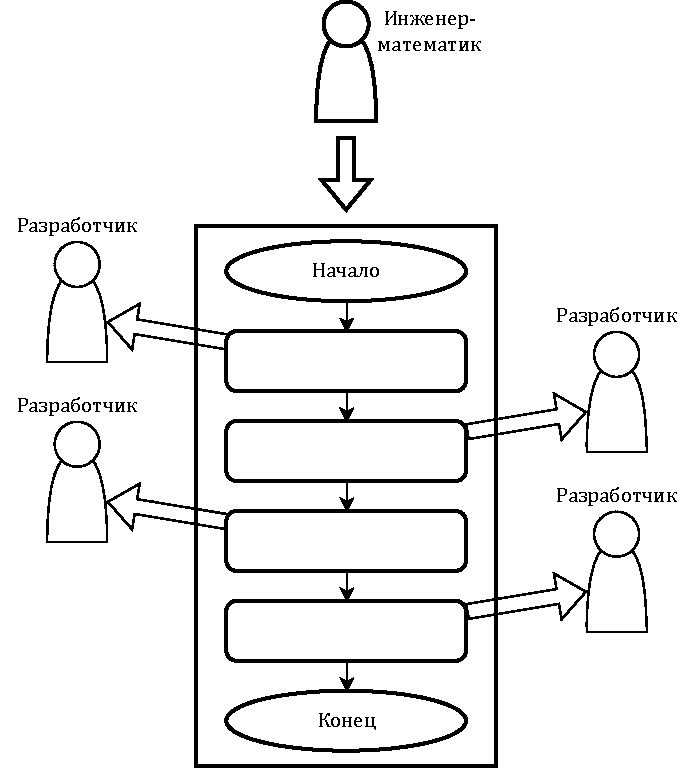
\includegraphics[height=0.6\textheight]{images/illustration.teamwork.pdf}
    \end{minipage}\hfill\begin{minipage}{0.49\textwidth}
      \begin{itemize}
        \item Введение новых разработчиков в проект влечёт за собой необходимость описывать для них логику реализуемого решения.
        \item Целесообразно включить разработку описания логики решения в процесс его программной реализации.
      \end{itemize}
    \end{minipage}\hfill
  \end{figure}

\end{frame}


% --------------------------------------------------------------------------- %
\subsection{Современные средства, направленные на упрощение реализации решений прикладных задач}
% --------------------------------------------------------------------------- %
\begin{frame}

  {\smaller[1]
    Среди современных средств упрощения разработки можно выделить следующие:
    \begin{itemize}
      \item научные системы управления потоком задач.
      \item платформы малокодовой разработки (LCPD).
    \end{itemize}
  }

  \begin{block}{Основной принцип}
    \smaller[1]
    Использование формальных описаний алгоритма решения при его непосредственной программной реализации.
  \end{block}

  \begin{figure}
    \begin{minipage}{0.49\textwidth}
      \centering
      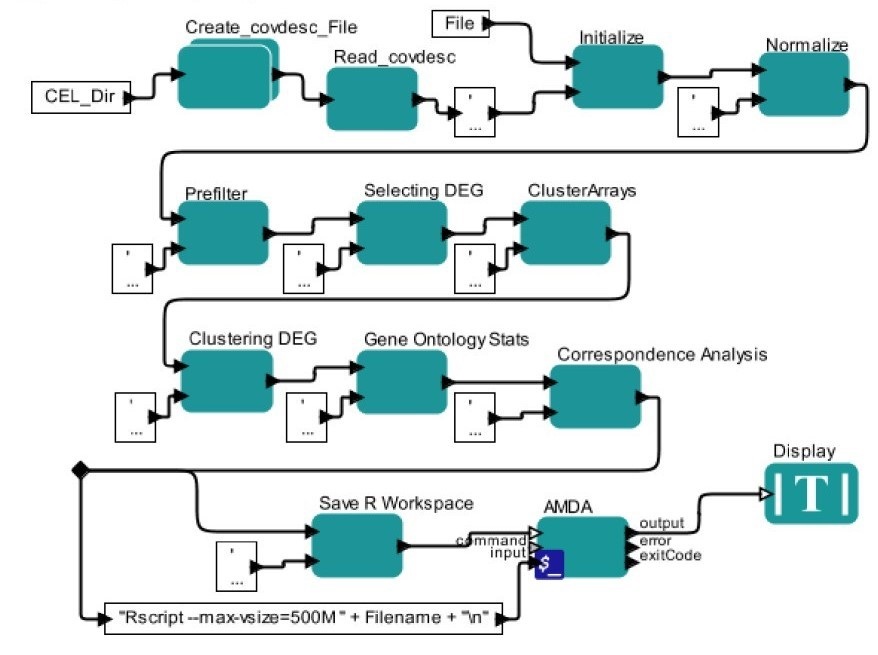
\includegraphics[width=\textwidth]{images/screenshot.KeplerWorkflow.jpg}
      \caption{\smaller[1] Пример описания алгоритма в научной системе управления потоком задач Kepler}
    \end{minipage}\hfill\begin{minipage}{0.49\textwidth}
      \centering
      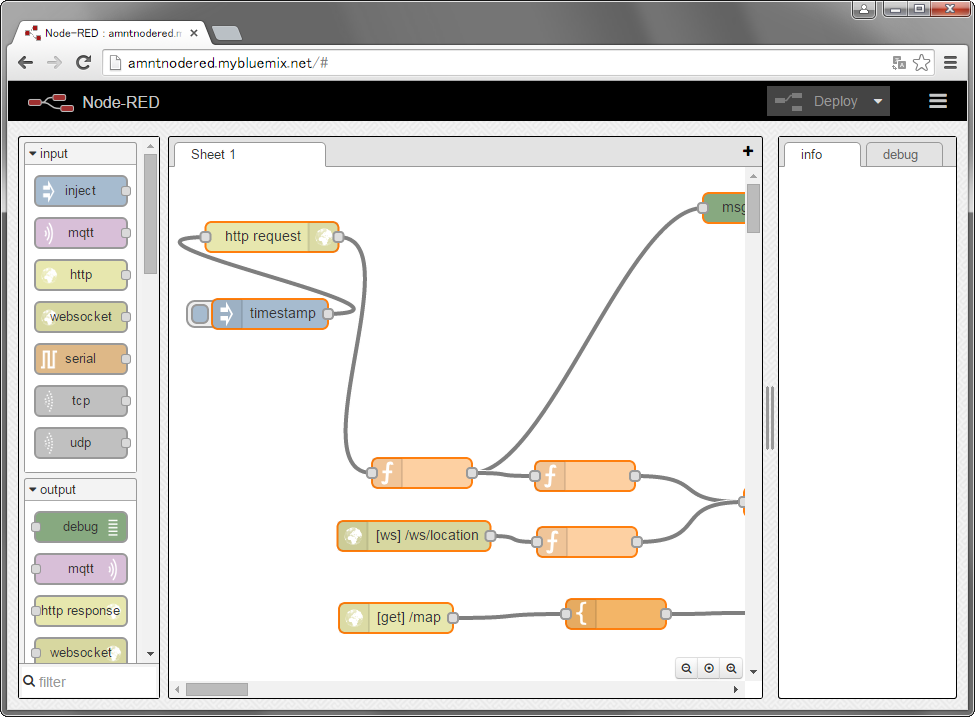
\includegraphics[width=\textwidth]{images/screenshot.NodeRED.png}
      \caption{\smaller[1] Пример описания алгоритма в LCPD Node-RED}
    \end{minipage}\hfill
  \end{figure}
\end{frame}

% --------------------------------------------------------------------------- %
\subsection{Подходы к построению формальному описанию логики процесса}
% --------------------------------------------------------------------------- %
\begin{frame}
  \begin{itemize}
    \item Можно выделить следующие подходы:
          \begin{itemize}
            \item Диаграммы потоков данных (DFD).
            \item Диаграммы потока управления.
            \item Диаграммы переходов состояний.
          \end{itemize}

    \item \textbf{Рассматриваемый в данной работе подход GBSE является частным случаем применения диаграмм переходов состояний.}
  \end{itemize}

\end{frame}




%---------------------------------------------
% --------------------------------------------------------------------------- %
\subsection{Диаграммы потоков данных}
% --------------------------------------------------------------------------- %
\begin{frame}
    Описание алгоритма -- ориентированный граф. В его вершинах -- процессы обработки данных, рёбра -- пути данных между процессами.

    \begin{figure}
        \centering
        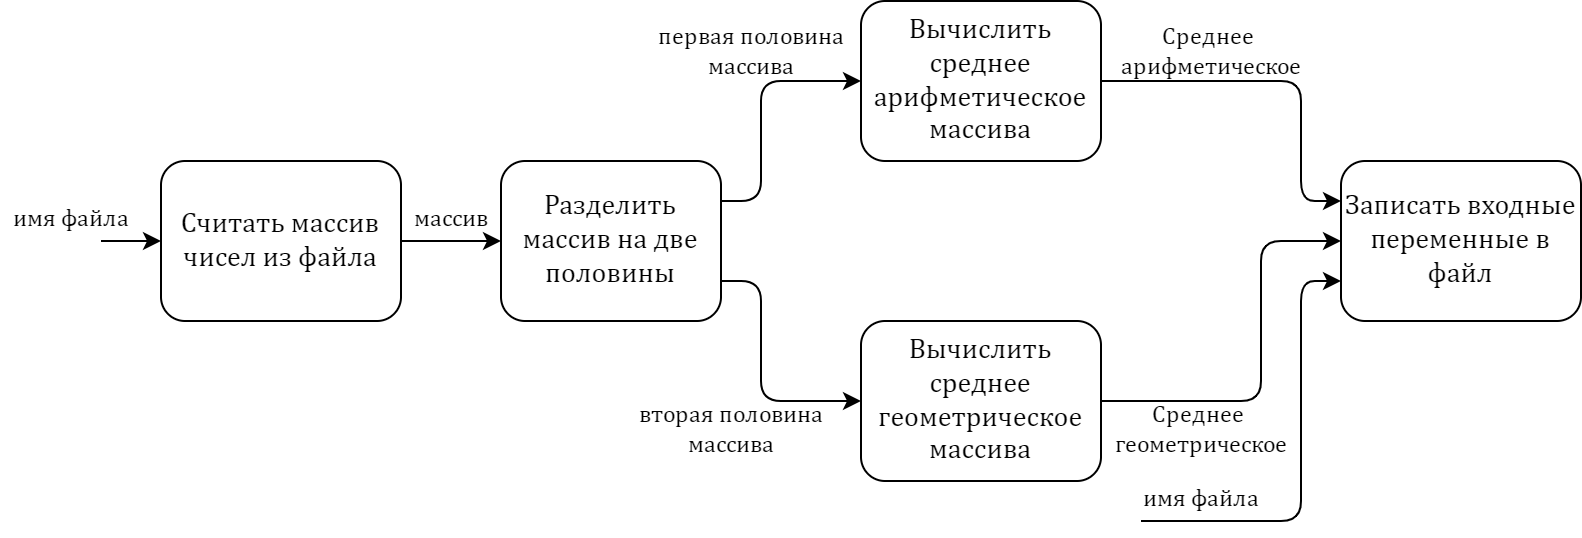
\includegraphics[width=0.8\textwidth]{images/illustration.dataflow.png}
        \caption{Пример диаграммы потоков данных, описывающей вычисление среднего арифметического и среднего геометрического двух половин массива целых чисел с последующей записью результатов в файл}
    \end{figure}

\end{frame}


\subsection{pSeven -- реализация диаграмм потоков данных}
%%%%%%%%%%%%%%%%%%%%%%%%%%%%%%%%%%%%%%%%%%%
\begin{frame}
    \begin{figure}
        \centering
        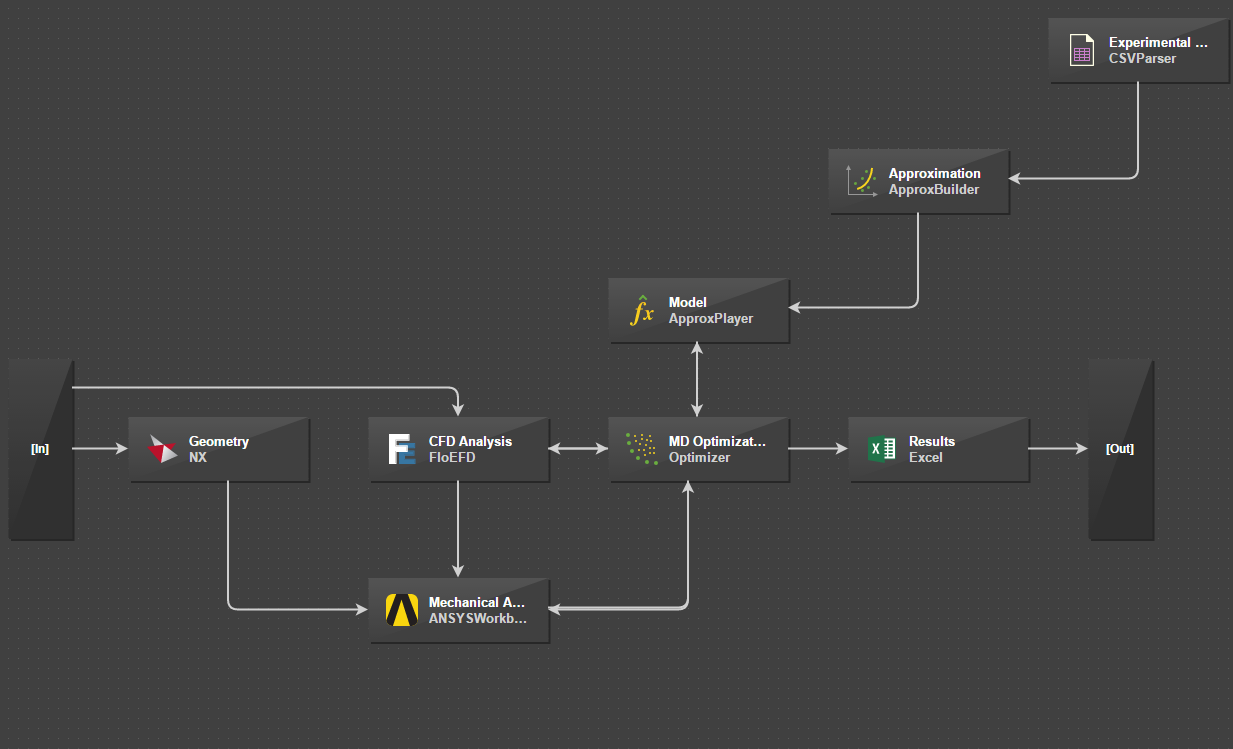
\includegraphics[width=\textwidth]{images/workflow1.png}
        \caption{Графический пользовательский интерфейс pSeven}
    \end{figure}

\end{frame}

% --------------------------------------------------------------------------- %
\subsection{Результаты сравнения. Выявленные достоинства объекта разработки}
% --------------------------------------------------------------------------- %
\begin{frame}
    Основные достоинства comsdk по сравнению с pSeven:
    \begin{itemize}
        \item Нет необходимости указывать входные и выходные данные при описании алгоритма.
        \item По умолчанию поддерживаются алгоритмы, подразумевающие взаимодействие с пользователем
    \end{itemize}

    \begin{figure}
        \centering
        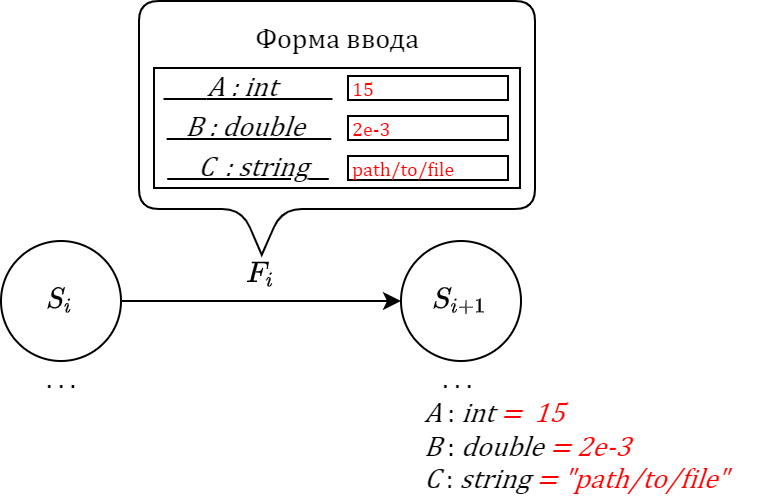
\includegraphics[height=0.33\textheight]{images/illustration.form_generation.png}
    \end{figure}

    \begin{itemize}
        \item Результат применения -- компилируемая программа с возможностью запуска на различных платформах.
    \end{itemize}
\end{frame}

% --------------------------------------------------------------------------- %
\subsection{Результаты сравнения. Выявленные недостатки объекта разработки}
% --------------------------------------------------------------------------- %
\begin{frame}
    Основные недостатки comsdk по сравнению с pSeven:
    \begin{itemize}
        \item Отсутствие поддержки матричных типов данных.
        \item Отсутствие средств визуализации результатов расчётов.
        \item Отсутствие возможности использования при расчётах распределённых вычислительных систем;
    \end{itemize}
\end{frame}
%%%%%%%%%%%%%%%%%%%%%%%%%%%%%%%%%%%%%%%%%%%
%---------------------------------------------
\section{Постановка задачи}
% --------------------------------------------------------------------------- %
\subsection{Состояния данных}
% --------------------------------------------------------------------------- %
\begin{frame}
	\begin{figure}
		\centering
		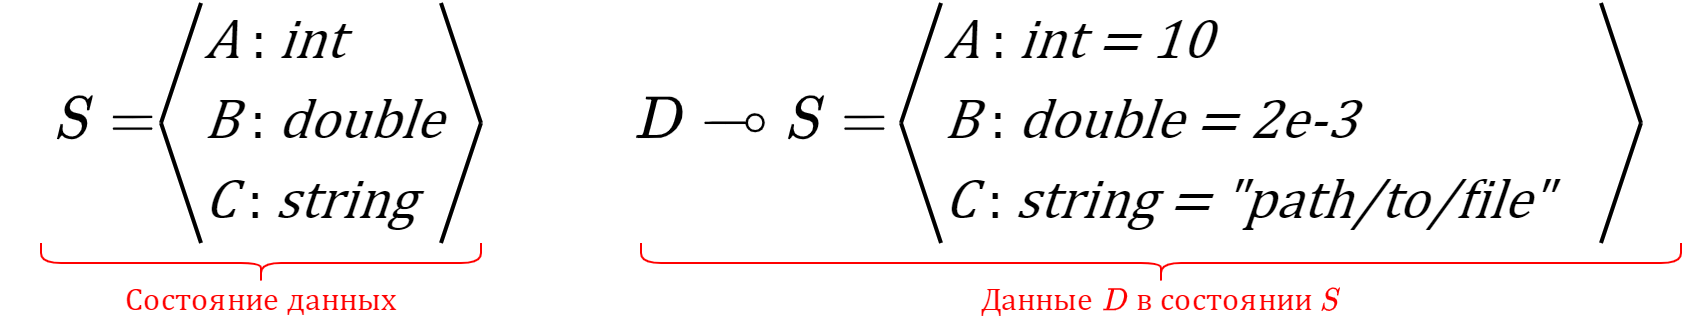
\includegraphics[width=\textwidth]{images/illustration.datastate.png}
	\end{figure}
	Состояние данных определяет, какие переменные какого типа должны быть определены на данном этапе алгоритма.

	Данные алгоритма модифицируются по ходу его выполнения.
\end{frame}

% --------------------------------------------------------------------------- %
\subsection{Функции-обработчики}
% --------------------------------------------------------------------------- %
\begin{frame}
	\begin{figure}
		\centering
		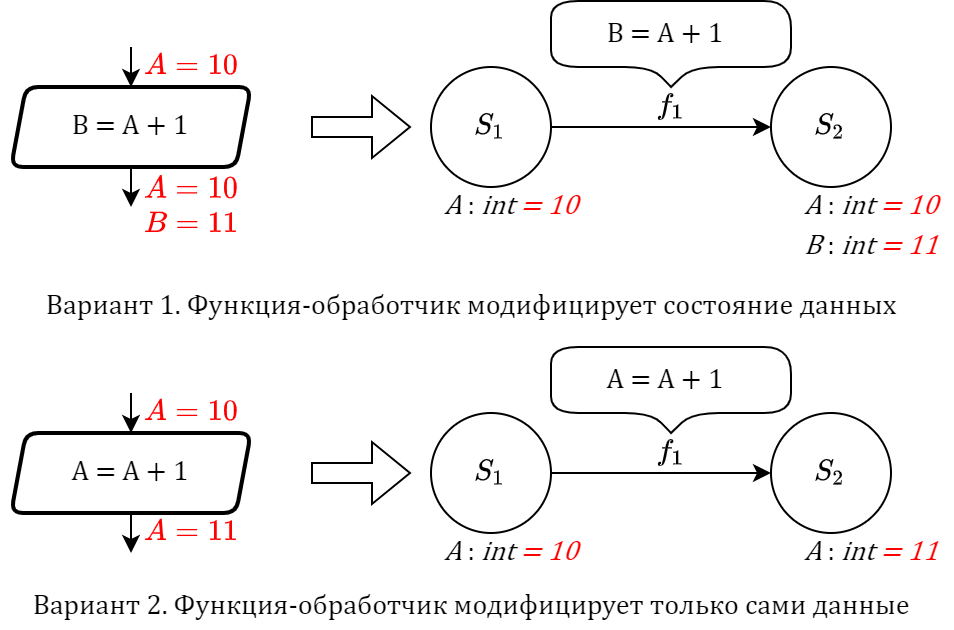
\includegraphics[width=0.7\textwidth]{images/illustration.transfer.png}
	\end{figure}

	Функции-обработчики отвечают за обработку данных и их перевод из одного состояния в другое.
\end{frame}


% --------------------------------------------------------------------------- %
\subsection{Функции-предикаты и функции перехода}
% --------------------------------------------------------------------------- %
\begin{frame}
	\begin{figure}
		\begin{minipage}{0.49\textwidth}
			\centering
			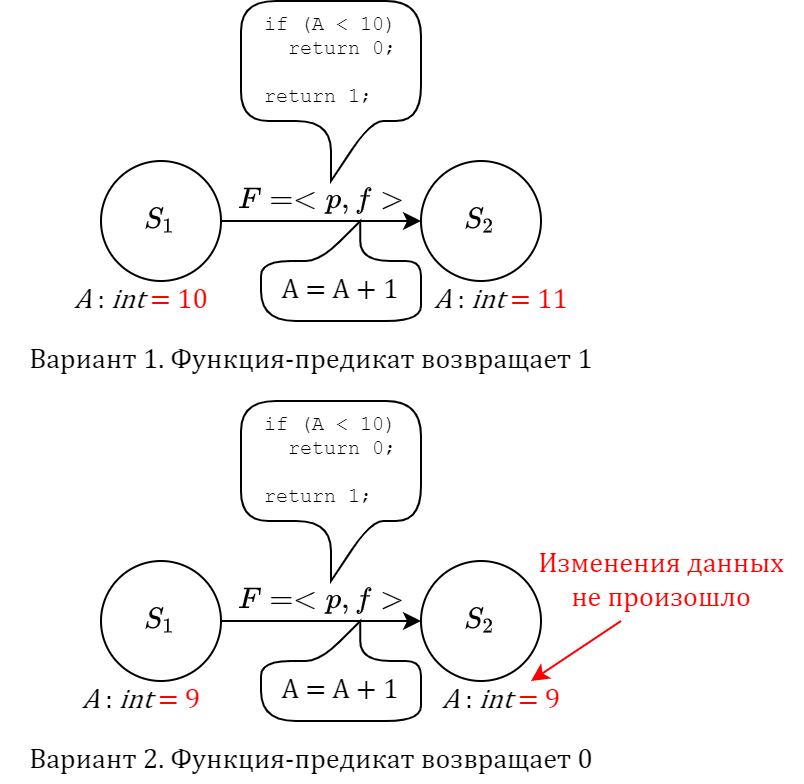
\includegraphics[height=0.5\textheight]{images/illustration.predicate.png}
			\caption{Принцип работы функции-предиката}
		\end{minipage}\hfill\begin{minipage}{0.49\textwidth}
			\centering
			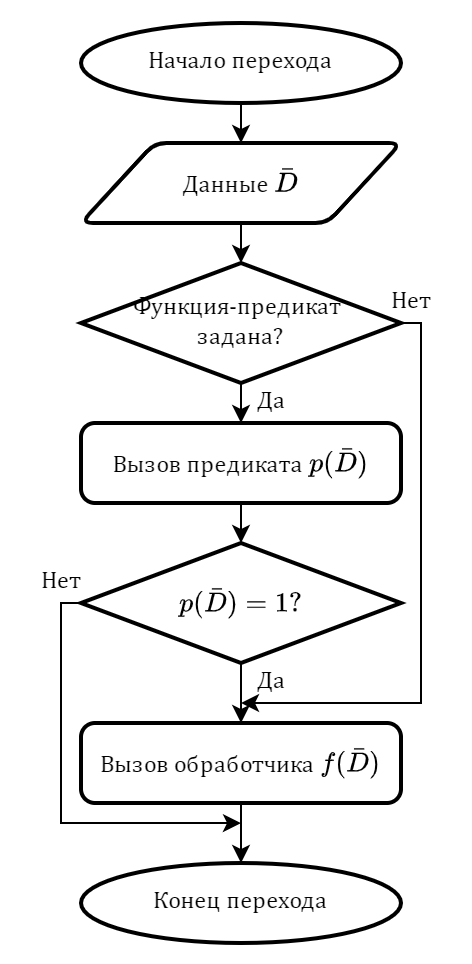
\includegraphics[height=0.5\textheight]{images/flowchart.Transfer.png}
			\caption{Блок-схема логики функции перехода}
		\end{minipage}\hfill
	\end{figure}

	Функции-предикаты отвечают за предварительную проверку данных перед их обработкой.

	Функция перехода -- составная функция $F=<p,f>$, содержащая в себе функцию-предикат $p$ и функцию-обработчик $f$.
\end{frame}

% --------------------------------------------------------------------------- %
\subsection{Функции-селекторы}
% --------------------------------------------------------------------------- %

\begin{frame}
	Функции-селекторы отвечают за проверку условий при ветвлении алгоритма.

	\begin{figure}
		\centering
		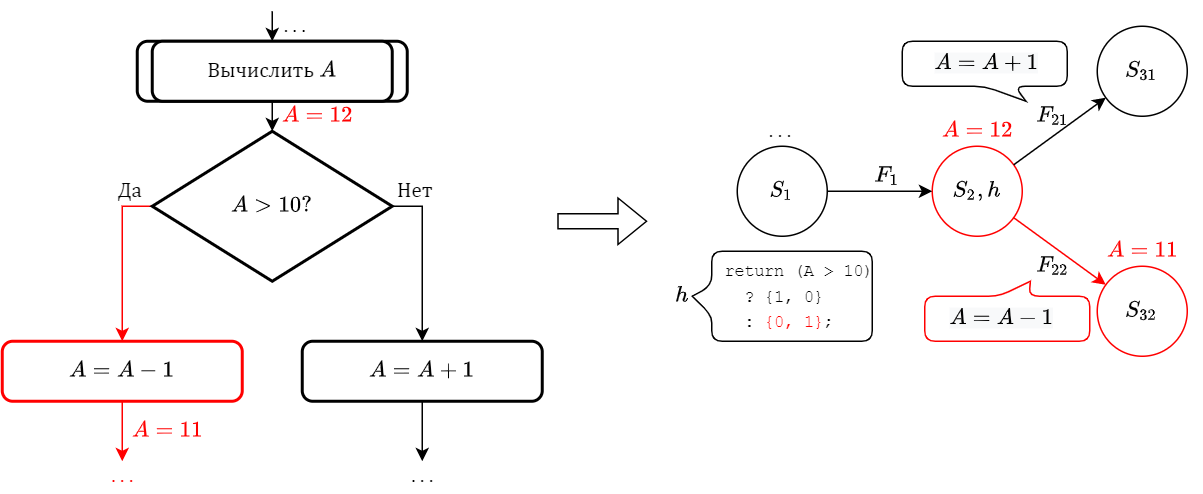
\includegraphics[width=0.9\textwidth]{images/illustration.selector.png}
		\caption{Принцип работы функций-селекторов. $h$ -- функция селектор. Красным показана ветвь алгоритма, которая будет выполнена.}
	\end{figure}
\end{frame}

% --------------------------------------------------------------------------- %
\subsection{Графовая модель}
% --------------------------------------------------------------------------- %
\begin{frame}
	Графовая модель сложного вычислительного метода описывает его логику в виде ориентированного графа, где узлам ставятся в соответствие состояния данных, а рёбрам -- функции перехода.

	\begin{figure}
		\centering
		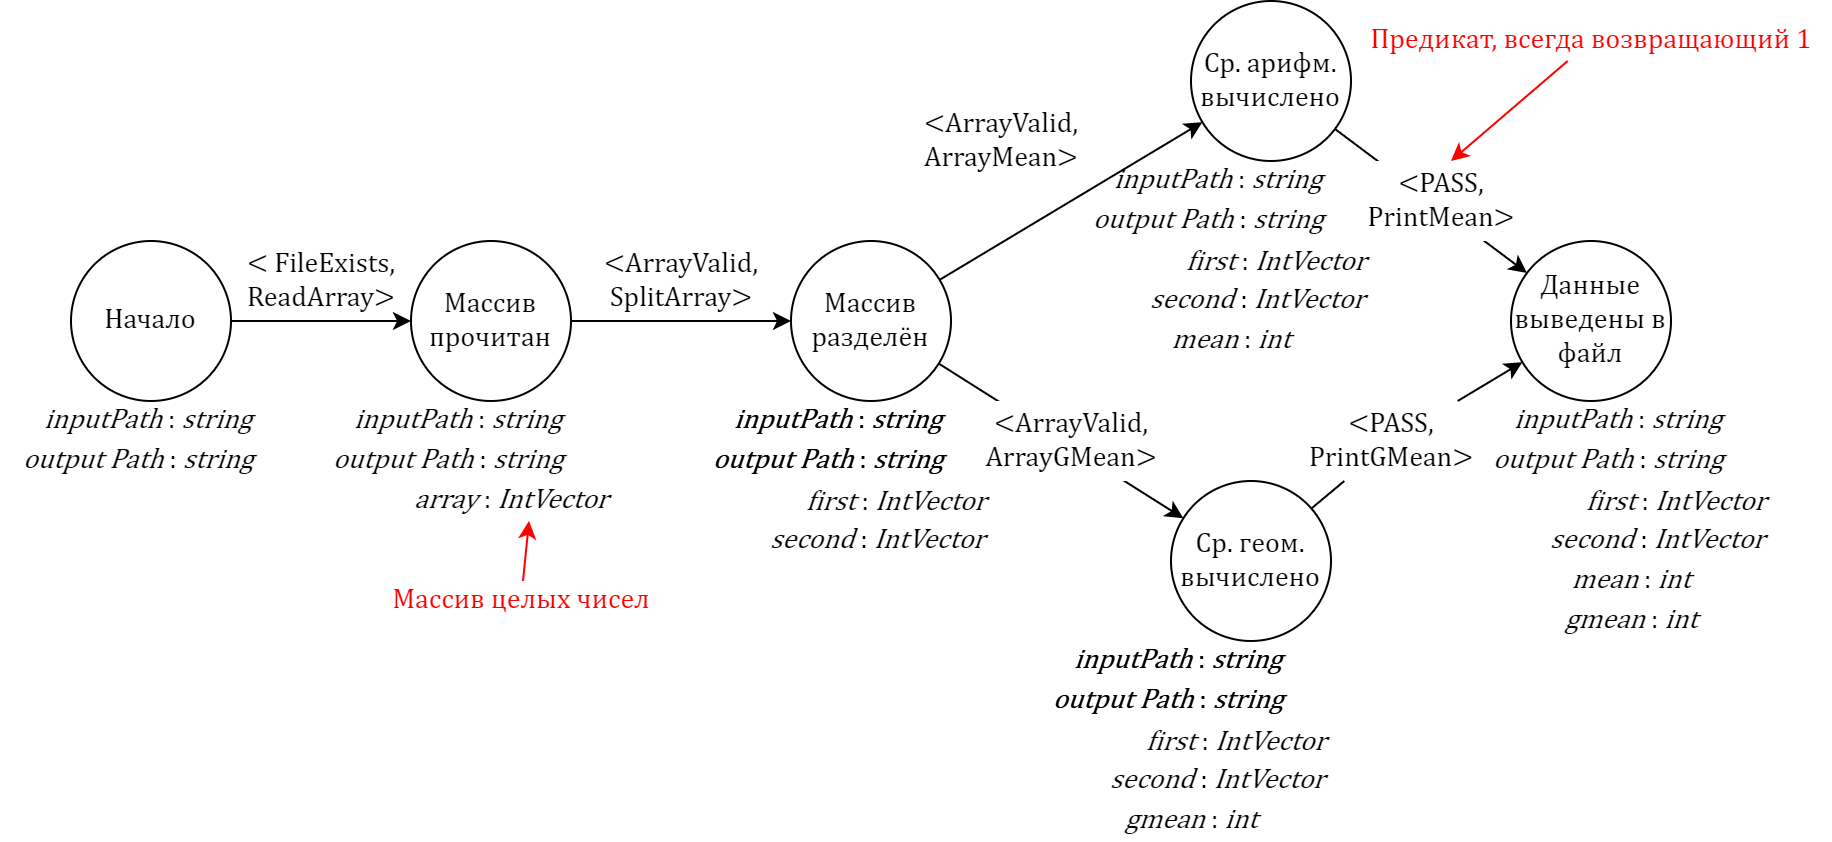
\includegraphics[width=\textwidth]{images/illustration.graph.png}
		\caption{Пример графовой модели, описывающей вычисление среднего арифметического и среднего геометрического двух половин массива целых чисел с последующей записью результатов в файл}
	\end{figure}

\end{frame}

\begin{frame}
	\begin{figure}
		\begin{minipage}{0.49\textwidth}
			\centering
			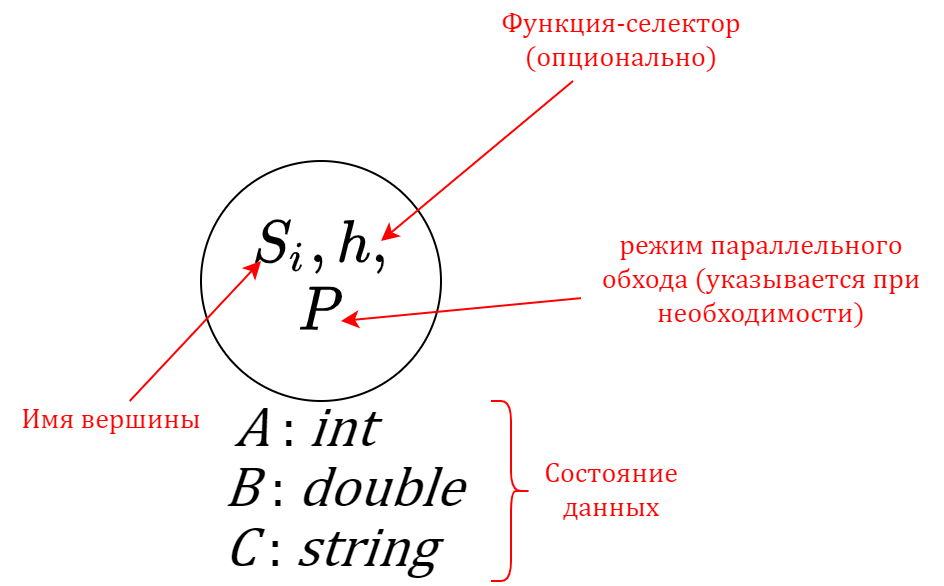
\includegraphics[width=0.49\textwidth]{images/illustration.node.png}
		\end{minipage}\hfill\begin{minipage}{0.49\textwidth}
			Атрибуты вершины:
			\begin{enumerate}
				\item имя;
				\item состояние данных;
				\item селектор;
				\item режим параллельного обхода исходяших ветвей
			\end{enumerate}
		\end{minipage}\hfill
	\end{figure}
\end{frame}

%---------------------------------------------
\section{Программная реализация}
% --------------------------------------------------------------------------- %
\subsection{Функциональные структуры данных}
% --------------------------------------------------------------------------- %
\begin{frame}
    \begin{figure}
        \smaller[1]
        \centering
        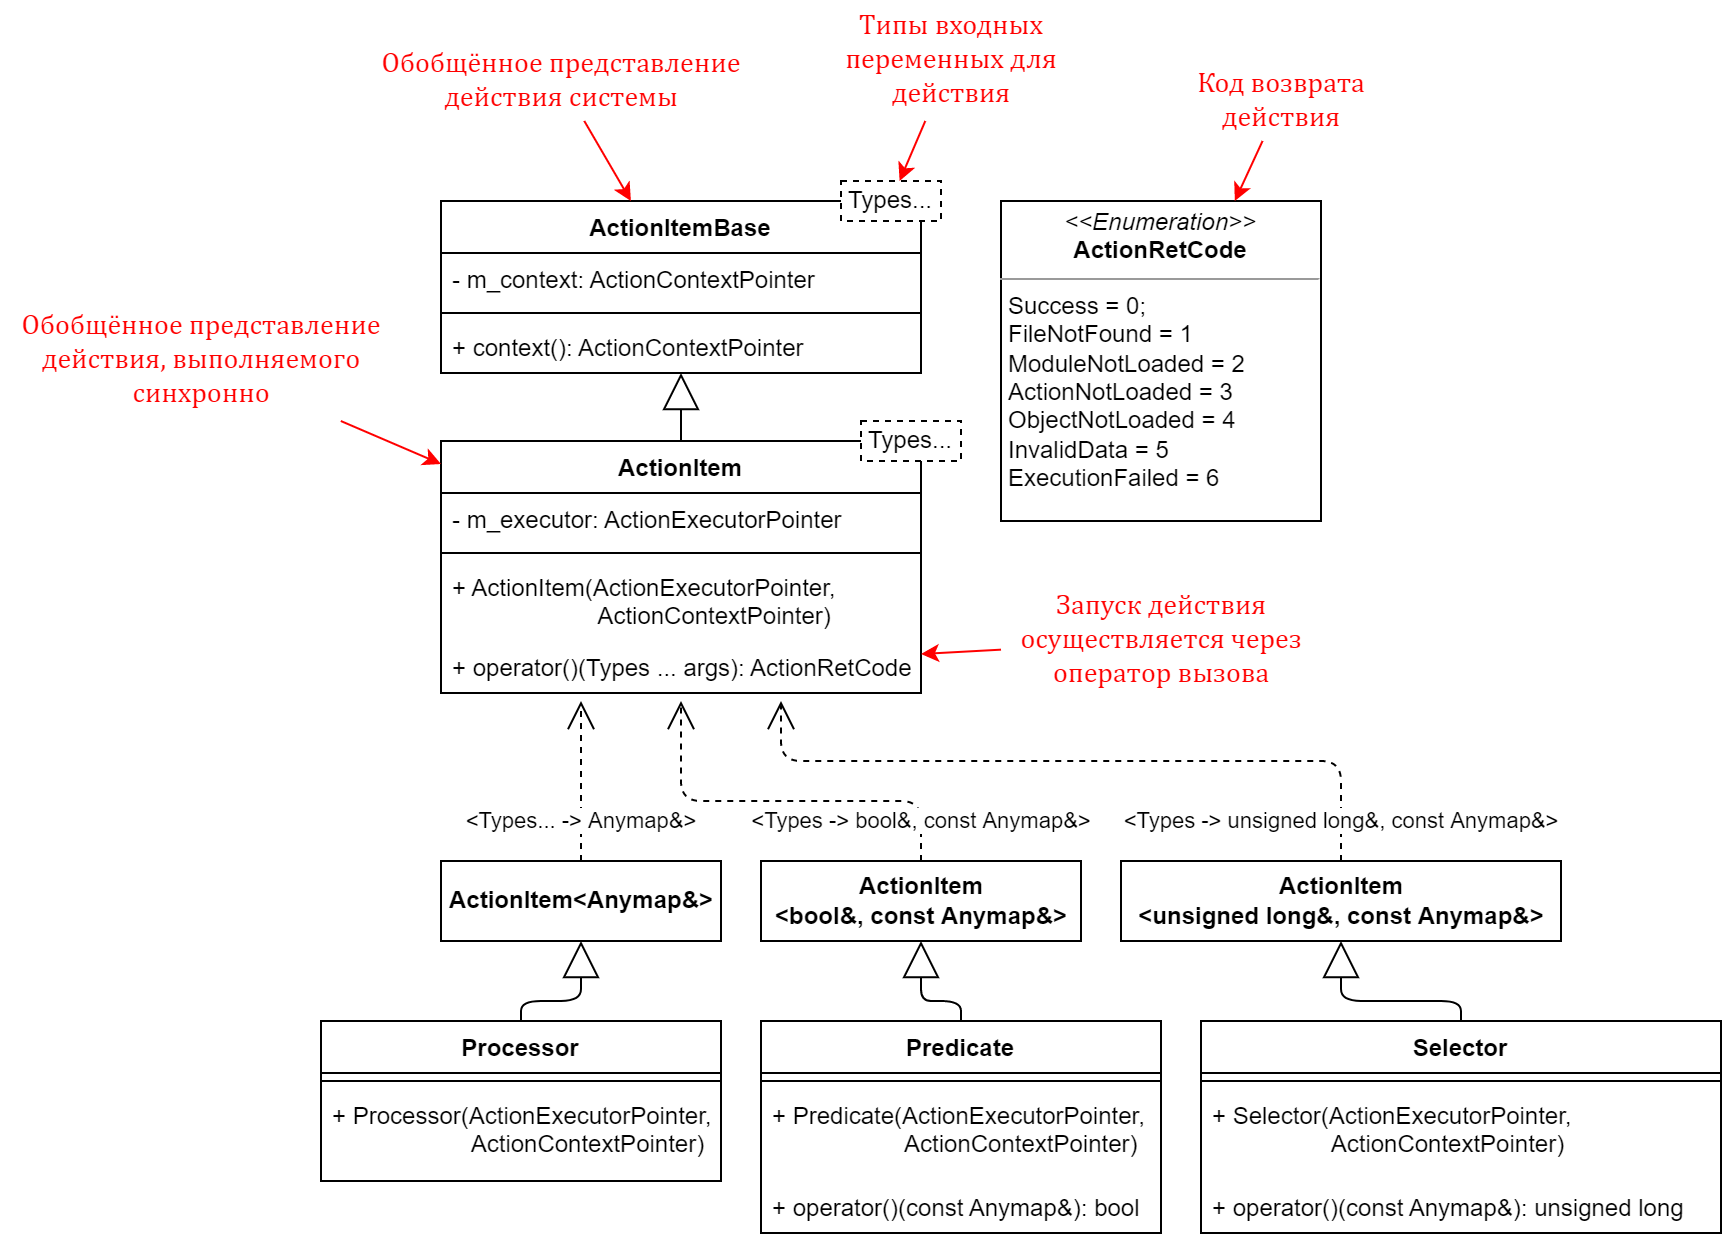
\includegraphics[height=0.75\textheight]{images/UML.graphFunctions.png}
        \caption{UML-диаграмма разработанных структур данных, отвечающих за представление функций-предикатов, обработчиков и селекторов}
    \end{figure}

\end{frame}
% --------------------------------------------------------------------------- %
\subsection{Информационные структуры данных}
% --------------------------------------------------------------------------- %
\begin{frame}

\end{frame}
% --------------------------------------------------------------------------- %
\subsection{Требования к алгоритму обхода}
% --------------------------------------------------------------------------- %
\begin{frame}
    \begin{figure}
        \centering
        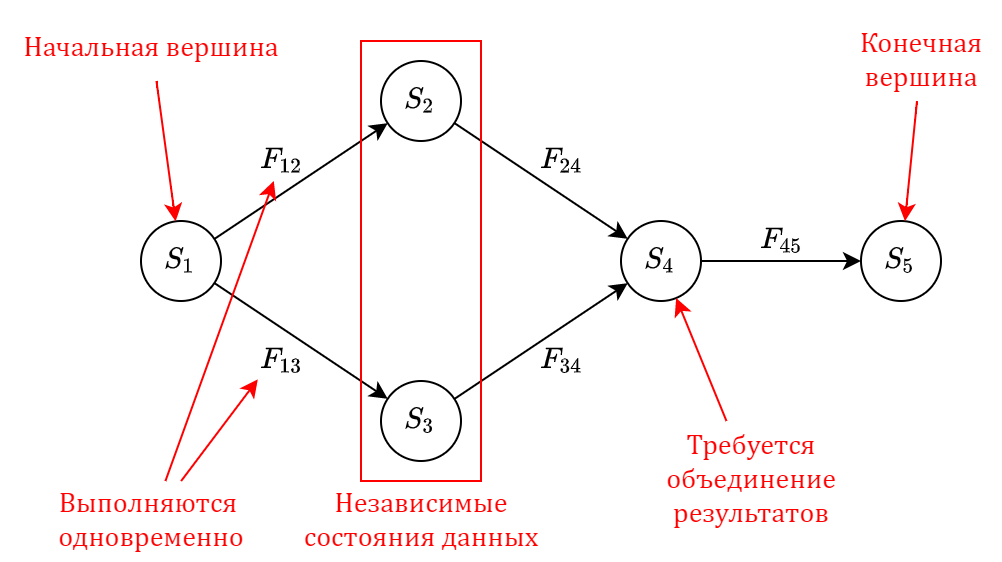
\includegraphics[width=0.6\textwidth]{images/illustration.parallel_run.png}
        \caption{Пример графовой модели, подразумевающей паралельный обход ветвей}
    \end{figure}

    Режим параллельного исполнения в вершине $S_1$ определяет, какие ресурсы будут задействованы для выполнения ветвей $S_1 \to S_2 \to S_4$ и $S_1 \to S_3 \to S_4$
\end{frame}

% --------------------------------------------------------------------------- %
\subsection{Управляющие структуры данных}
% --------------------------------------------------------------------------- %
\begin{frame}


\end{frame}
% --------------------------------------------------------------------------- %


%---------------------------------------------
\section*{Заключение}
%%%%%%%%%%%%%%%%%%%%%%%%%%%%%%%%%%%%%%%%%%%
%\subsection{}
%\def\subsecname{}
%%%%%%%%%%%%%%%%%%%%%%%%%%%%%%%%%%%%%%%%%%%
% --------------------------------------------------------------------------- %
\subsection*{Анализ результатов}
% --------------------------------------------------------------------------- %
\begin{frame}%[allowframebreaks=0.9,t]

	В результате выполнения работы:
	\begin{enumerate}[1)]
		\item расширены функциональные возможности библиотеки comsdk
		\item создана новая архитектура классов, позволяющая в дальнейшем упростить процесс автоматического формирования программного представления графовых моделей;
		\item разработаны структуры данных для программного представления графовых моделей алгоритмов и их элементов;
		\item был разработан алгоритм, осуществляющий выполнение этапов алгоритма в соответствии с его графовой моделью;
	\end{enumerate}

\end{frame}
% --------------------------------------------------------------------------- %
\subsection*{Перспективы разработки}
% --------------------------------------------------------------------------- %
\begin{frame}
	Перспективы развития программного каркаса comsdk включают в себя:
	\begin{itemize}
		\item реализации алгоритма обхода графовой модели с задействованием различных вычислительных ресурсов
		\item интеграцию средства генерации форм ввода\footcite{SokolovPershin2017};
		\item разработку средства визуализации обрабатываемых данных;
		\item разработку средства автоматической документации реализуемых алгоритмов;
	\end{itemize}

\end{frame}

%%%%%%%%%%%%%%%%%%%%%%%%%%%%%%%%%%%%%%%%%%%

%---------------------------------------------
\def\secname{}

\begin{frame}

    \begin{center}
        \LARGE
        Спасибо за внимание!
    \end{center}

\end{frame}
%---------------------------------------------
\end{document}
%---------------------------------------------



